\chapter{Discussione, limiti e minacce alla validità}
\label{sec:discussion}

% Source notes: Project/docs/thesis_notes.md, checkpoint_2026-10-10.md (takeaways and caveats).

Questo capitolo interpreta i risultati alla luce delle cinque domande di ricerca. Indica poi ciò che gli esperimenti non
possono dimostrare e quali scelte potrebbero averli distorti.

\section{Quando conviene un Decision Model specialista}
\label{sec:disc-synthesis}

\paragraph{Specializzazione (RQ1).} A rendere GroundOne accurato è l'addestramento sulla decisione. I modelli non
addestrati restano vicini al caso, mentre gli stessi modelli, una volta addestrati, raggiungono sul test set di RAGTruth
una balanced accuracy a tre classi di 0.769 (0.5B) e 0.832 (3B). Superano così gli encoder specializzati in AUROC, e
Rizzo-Flow, un decision model generalista otto volte più grande, in balanced accuracy a tre classi. Il vantaggio, però, si
concentra dove si trovano i dati di addestramento. Su LLM-AggreFact il 3B si porta alla pari con il miglior encoder di
piccole dimensioni, senza superarlo, e resta sotto il decision model chiuso Jev e un modello open da 27B, misurati in modo
indipendente; il 0.5B rimane al di sotto dell'encoder. Su VitaminC, infine, il 3B addestrato non fa meglio di quello non
addestrato.

Il confronto con d1-3B, un decision model generalista della stessa dimensione, rende esplicito il compromesso. d1-3B è già
addestrato a decidere, ma su un'ampia miscela di task. Su RAGTruth è molto lontano da GroundOne, soprattutto sulle
risposte lunghe; su LLM-AggreFact è alla pari con il 3B; su VitaminC è nettamente superiore. Uno specialista è dunque una
scelta solida per il dominio su cui è stato addestrato, ma uno strumento debole per la verifica dei fatti in generale.
All'interno del dominio la specializzazione garantisce accuratezza e robustezza sulle risposte lunghe, a scapito del
trasferimento; fuori dal dominio, invece, sono la dimensione del modello oppure un'ampia miscela di addestramento a
migliorare il trasferimento.

\paragraph{Readout e generazione a confronto (RQ2).} Il meccanismo del decision model contribuisce in due modi distinti. Il primo
riguarda il costo: un solo forward pass sulla risposta sostituisce la generazione di $K$ verdetti, per cui il tempo
risparmiato cresce con la lunghezza della risposta. Quando la risposta contiene quattordici o più frasi, il risparmio
arriva a un fattore di circa due rispetto a un giudice sintetico e di circa sei rispetto a uno verboso. Il secondo
contributo, che questa tesi non aveva previsto, riguarda l'accuratezza. Con gli stessi pesi e lo stesso costo, scegliere
tra le tre lettere ammissibili è più accurato che prendere il token che il modello genererebbe, con un guadagno di
balanced accuracy a tre classi di 0.25 per il 0.5B e di 0.07 per il 3B. Un decision model sottoposto a fine-tuning si
comprende quindi meglio come un classificatore a tre classi innestato su un modello linguistico che come un generatore
che si ferma dopo un token. La distinzione pesa soprattutto per i modelli piccoli, cioè proprio per quelli che un
portatile può permettersi. Il confronto con i giudici generativi, infine, misura anche l'effetto dell'addestramento:
poiché i giudici non sono addestrati, le ampie differenze di accuratezza rispetto a GroundOne vanno lette come l'effetto
congiunto della specializzazione e del readout. La Figura~\ref{fig:disc-gains} scompone il guadagno su T1 nei due passaggi, l'addestramento e il readout ristretto.

\begin{figure}[htbp]
\centering
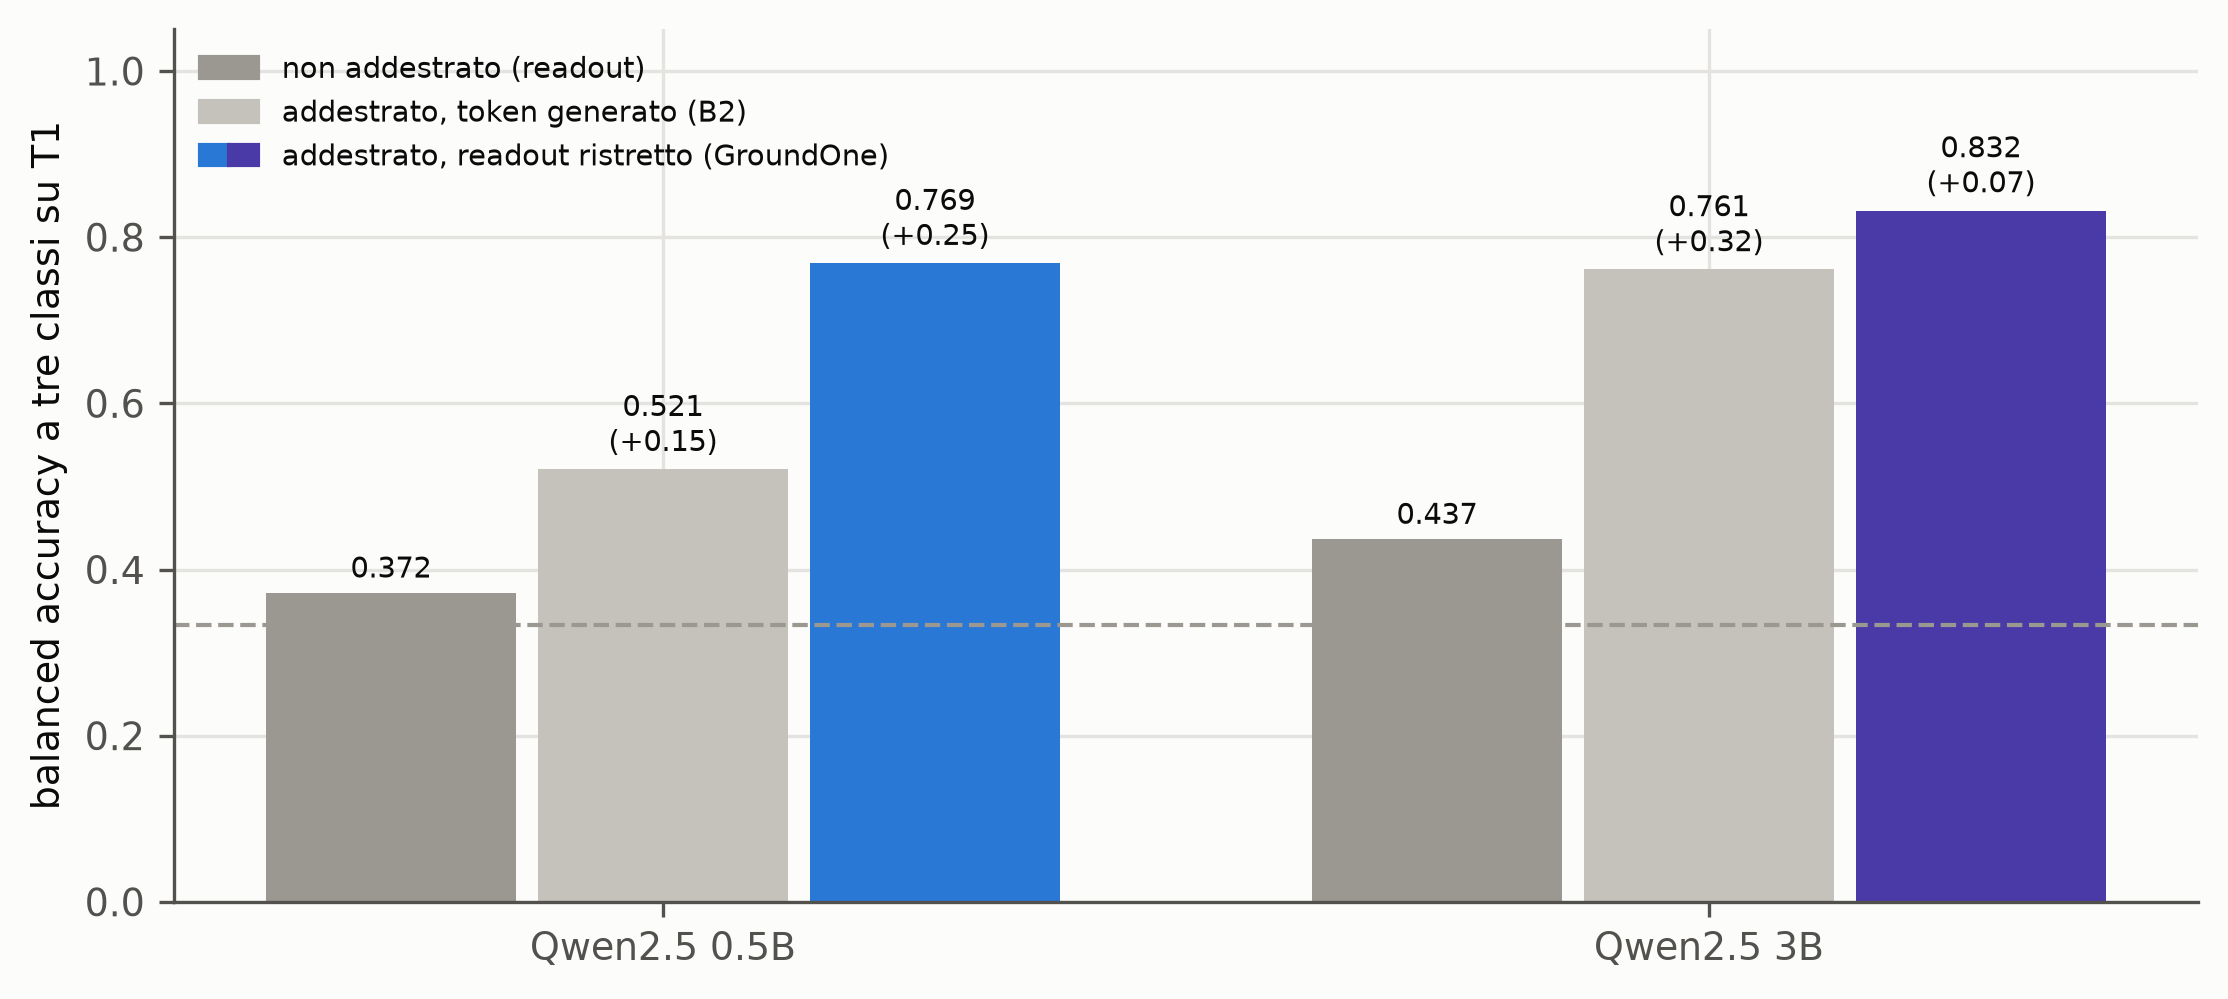
\includegraphics[width=\textwidth]{images/results/gain_decomposition.png}
\caption{Da dove viene l'accuratezza di GroundOne su T1: lo stesso modello base non addestrato (readout, design a), addestrato ma con la decisione presa dal token che genererebbe (controllo B2, errori di formato contati come errori) e addestrato con il readout ristretto. Tra parentesi il guadagno rispetto al passaggio precedente. Il 3B non addestrato è valutato su 600 risposte; il tratteggio indica il livello casuale.}
\label{fig:disc-gains}
\end{figure}

\paragraph{Calibrazione (RQ3).} Una temperatura e un bias stimati sul dev set allineano le probabilità alle frequenze
osservate sul test set dello stesso dominio, e le probabilità calibrate rendono efficace la selective prediction. Due
indicazioni valgono al di là di GroundOne. La prima è che l'Expected Calibration Error, da solo, non basta a ordinare i
sistemi. Dopo la stessa calibrazione, giudici le cui probabilità separano a malapena le classi raggiungono lo stesso ECE
di GroundOne, e soltanto l'AUROC e la risk--coverage curve ne rivelano la differenza. La seconda è che decisioni e
probabilità vanno ricavate in modo coerente. Se si sceglie la classe calibrata più probabile, la decisione collassa verso
la classe maggioritaria; una soglia stimata sul dev set, invece, recupera la decisione bilanciata e mantiene l'etichetta
coerente con la probabilità mostrata all'utente. Come mostrano i risultati su VitaminC, infine, la calibrazione vale
soltanto per la distribuzione su cui è stata stimata.

\paragraph{Costo sul dispositivo (RQ4).} Il verificatore sta comodamente nel portatile da 16\,GB. Durante
l'addestramento la memoria occupata raggiunge un picco di 2.6\,GB con il 0.5B e di 5.9\,GB con il 3B. Verificare una
risposta lunga richiede 0.41 secondi e 5.5 joule con il 0.5B, 2.57 secondi e 33 joule con il 3B. Il 0.5B rientra in un
budget interattivo; il 3B, invece, su una risposta tipica è più lento di quanto un uso interattivo richiederebbe, e
scambia tempo con accuratezza. Le misure di energia precisano la portata dei risultati sulla velocità. Un singolo
prefill lungo assorbe più potenza del decoding token per token, per cui l'energia risparmiata è inferiore al tempo
risparmiato, e la maggiore velocità non va letta come un risparmio equivalente di batteria. Il verificatore convive
inoltre con un generatore nello stesso processo: insieme a un generatore 3B a 4 bit, il picco di memoria è di 6.1\,GB con
il 3B e di 3.3\,GB con il 0.5B. L'intera valutazione gira senza alcun accesso alla rete, con risultati identici bit per
bit, e i pesi a 8 bit non costano accuratezza rispetto a quelli in bf16 (Sezione~\ref{sec:results-locality}). Resta da
misurare il retriever, che verrà valutato nell'applicazione dimostrativa.

Anche il costo economico va letto con misura (Tabella~\ref{tab:disc-cost}). Verificare 10{,}000 risposte con
GroundOne richiede un'energia che, al prezzo medio europeo dell'elettricità per le famiglie~\cite{eurostat2026electricity},
vale meno di un centesimo di euro con il 0.5B e circa tre centesimi con il 3B. Affidare la stessa verifica a un giudice
in cloud, ai prezzi di listino dei fornitori~\cite{anthropic2026pricing,openai2026pricing,google2026geminipricing},
costa invece da circa un dollaro con i modelli più economici a oltre duecento con quelli di fascia più alta. Il rapporto
è quindi di due-quattro ordini di grandezza, ma in valore assoluto i giudici economici restano poco costosi, e il
confronto non considera né l'acquisto dell'hardware né la qualità dei giudici in cloud, che questa tesi non ha
misurato. L'argomento decisivo a favore della verifica locale resta quindi l'indipendenza: i documenti non lasciano la
macchina e il servizio non dipende da un fornitore esterno.

\begin{table}[htbp]
\centering
\caption{Costo indicativo della verifica di 10{,}000 risposte RAG. Giudici in cloud: prezzi di listino del livello
standard, consultati il 19 ottobre 2026, con circa 900 token in ingresso per risposta (documento e risposta mediani di T1
più le istruzioni) e i token in uscita misurati per i giudici 3B di questa tesi (36 per il giudice sintetico, 248 per
quello verboso). GroundOne: energia netta misurata del chip moltiplicata per il prezzo medio dell'elettricità per le
famiglie nell'UE (0.29~€/kWh, secondo semestre 2025). Sono esclusi il costo dell'hardware e gli sconti per caching o
elaborazione in batch.}
\label{tab:disc-cost}
\small
\begin{tabular}{lccc}
\toprule
Sistema & \makecell{Prezzo ingresso / uscita\\(USD per Mtoken)} & \makecell{Giudice\\sintetico} & \makecell{Giudice\\verboso} \\
\midrule
\makecell[l]{Claude Haiku 5.5,\\gpt-6-luna} & 0.10 / 0.50 & 1.1 USD & 2.2 USD \\
Gemini 3.5 Flash-Lite & 0.30 / 2.50 & 3.6 USD & 8.9 USD \\
Gemini 3.8 Flash & 0.75 / 3.75 & 8.2 USD & 16 USD \\
\makecell[l]{Claude Sonnet 5.5, gpt-6.1-sol,\\Gemini 4 Argon} & 2.00 / 10.00 & 22 USD & 43 USD \\
Claude Opus 5.5 & 4.00 / 20.00 & 43 USD & 86 USD \\
gpt-6-astra & 10.00 / 50.00 & 109 USD & 215 USD \\
\midrule
GroundOne 0.5B (locale) & \multicolumn{3}{c}{0.015 kWh, circa 0.004 €} \\
GroundOne 3B (locale) & \multicolumn{3}{c}{0.092 kWh, circa 0.03 €} \\
\bottomrule
\end{tabular}
\end{table}

\paragraph{Oltre un punteggio binario (RQ5).} L'output a tre classi distingue bene le frasi contraddette da quelle non
menzionate nel data-to-text, il task in cui RAGTruth concentra le proprie contraddizioni. Le distingue molto meno nel
question answering e nella summarization, dove nei dati di addestramento le contraddizioni sono rare. Il 3B migliora
sensibilmente su questo fronte, e ciò suggerisce che al modello piccolo manchino, più che un'architettura diversa,
contraddizioni più varie in addestramento. Le policy strict e lenient e la soglia derivano tutte dalle stesse tre
probabilità. L'utente può quindi cambiare la nozione di errore senza riaddestrare il modello, cosa che nessun
verificatore binario consente. La Figura~\ref{fig:disc-when} riassume queste indicazioni in forma di albero decisionale.

\begin{figure}[htbp]
\centering
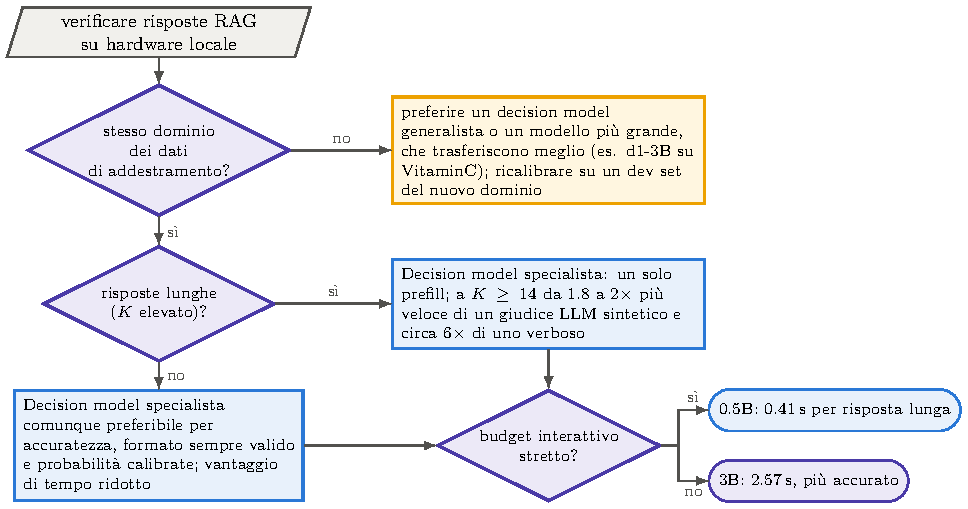
\includegraphics[width=\textwidth]{images/diagrams/disc_when_specialist_tikz.pdf}
\caption{Quando conviene un decision model specialista, secondo i risultati di questa tesi. È una sintesi qualitativa: i tempi si riferiscono al portatile M4 e alle risposte con 14 o più frasi, e il trasferimento fuori dominio è quello osservato su LLM-AggreFact e VitaminC.}
\label{fig:disc-when}
\end{figure}

\section{Limiti}
\label{sec:disc-limitations}

\paragraph{Una sola piattaforma e una sola famiglia di modelli.} Tutti i risultati provengono da un unico portatile, un
unico runtime e un'unica famiglia di modelli. Latenza ed energia dipendono dall'hardware e dall'implementazione: ciò che
dovrebbe valere anche altrove sono i rapporti tra i metodi, non i valori assoluti. La latenza di GroundOne non viene
confrontata con quella degli encoder né con quella dei decision model generalisti, perché questi sono stati eseguiti in
runtime diversi e in condizioni che renderebbero il confronto iniquo.

\paragraph{Stabilità dell'addestramento.} Due run completi del 0.5B concordano su tutte le metriche aggregate, ma un
terzo run è collassato nelle prime fasi ed è stato interrotto. La ricetta di addestramento non prevede gradient clipping
e usa AdamW senza bias correction, due cause note di fine-tuning
instabile~\cite{pascanu2013difficulty,mosbach2021stability}. L'una o l'altra potrebbe spiegare il collasso, ma nessuna
delle due ipotesi è stata verificata. Il 3B, inoltre, è stato addestrato una sola volta, su metà delle risposte di
addestramento, e la sua variabilità al cambiare del seed resta ignota.

\paragraph{Dati di addestramento.} RAGTruth è l'unica fonte di addestramento. Le sue contraddizioni sono concentrate nel
data-to-text e, al di fuori di questo task, vengono apprese solo in parte. I modelli, inoltre, si affidano in parte alla
sovrapposizione lessicale. Quando il supporto è espresso con parole diverse, la frase appare non supportata; quando una
frase copia la fonte salvo una piccola modifica, la modifica passa spesso inosservata. Questo punto cieco si riduce al
crescere del modello, ma resta il limite principale di entrambi.

\paragraph{Ambito della decisione.} La verifica avviene frase per frase e soltanto rispetto al documento recuperato. Una
frase vera nel mondo ma assente dal documento conta quindi come non menzionata: è il comportamento corretto per la
groundedness, ma non per la verifica dei fatti. Le frasi prive di contenuto verificabile vengono escluse da una regola, e
la segmentazione stessa può dividere o accorpare le affermazioni in modo diverso da un lettore umano. Infine, il verdetto
su una frase dipende soltanto dal documento e dalle frasi che la precedono.

\paragraph{Portata statistica.} Gli intervalli bootstrap descrivono la variabilità del test set, non quella
dell'addestramento. Inoltre, circa cinquanta confronti sono stati sottoposti a test senza correzione per confronti
multipli. Per questo le conclusioni poggiano su effetti ben lontani dallo zero, e non si rivendicano differenze su
LLM-AggreFact e VitaminC inferiori alla dispersione tra seed. Diverse baseline, infine, sono state valutate su
sottocampioni, il che ne allarga gli intervalli.

\section{Minacce alla validità}
\label{sec:disc-threats}

\paragraph{Etichette.} La distinzione tra frase contraddetta e non menzionata si basa sugli annotatori di RAGTruth, il
cui accordo sul tipo di allucinazione non è pubblicato. Inoltre, una recente riannotazione della partizione di test di
RAGTruth ha individuato un numero di risposte allucinate considerevolmente superiore a quello indicato dalle etichette
originali~\cite{yu2026retromorphic}. Il test set potrebbe quindi sottostimare le classi minoritarie. Per questo i
risultati a tre classi su RAGTruth vanno sempre letti insieme a quelli su VitaminC, le cui etichette hanno un accordo tra
annotatori misurato. LLM-AggreFact, infine, unifica le etichette di undici dataset di qualità diversa, e alcune delle sue
colonne sono notoriamente rumorose.

\paragraph{Vantaggio nel dominio.} GroundOne è addestrato su RAGTruth. I suoi risultati sul test set di RAGTruth e sulla
colonna RAGTruth di LLM-AggreFact lo avvantaggiano quindi rispetto a sistemi addestrati altrove. Per contro, VitaminC fa
parte dei dati da cui discende l'addestramento di MiniCheck-RoBERTa. Ogni confronto è riportato con la relativa
avvertenza, e le conclusioni poggiano sull'andamento complessivo nei tre test set anziché su uno solo.

\paragraph{Configurazione delle baseline.} I giudici generativi sono sensibili al prompt. I loro prompt sono stati
fissati prima di esaminare i risultati di test, e quello del giudice a parità di output è stato scelto sul dev set
unicamente in base alla validità del formato. Il parsing dell'output è stato permissivo, a vantaggio dei giudici. Il
decoding non era vincolato da una grammatica, e questo incide soprattutto sugli errori di formato del modello più
piccolo. Non sono stati valutati né un giudice sottoposto a fine-tuning sugli stessi dati né un giudice più grande: il
confronto misura dunque ciò che offre, senza addestramento, un giudice della stessa dimensione. Rizzo-Flow è stato
eseguito con pesi a 4 bit, perché il modello a 8 bit non trovava posto in memoria accanto al sistema operativo, e questo
potrebbe sottostimarne l'accuratezza. d1-3B, infine, è stato eseguito zero-shot e, su LLM-AggreFact, soltanto su un
sottocampione. Ha ricevuto le domande usate per tutte le baseline di tipo decision model, che potrebbero non essere la formulazione
a esso più congeniale.

\paragraph{Contaminazione.} I modelli base sono stati preaddestrati su ampi corpora web che potrebbero includere parti
dei test set pubblici\footnote{Si parla di \emph{contaminazione} dei dati quando esempi di un test set compaiono, anche
solo in parte, nei dati di preaddestramento di un modello. Un modello contaminato può ricordare gli esempi anziché
valutarli, e i suoi punteggi su quel test set risultano allora troppo ottimistici.}. Gli stessi modelli base, però,
usati senza addestramento come baseline, raggiungono un'accuratezza vicina al caso sul task a tre classi. La
contaminazione non può quindi spiegare i guadagni dovuti all'addestramento; per i valori assoluti, invece, non può essere
esclusa del tutto.

\paragraph{Una sola macchina.} Tutte le misure di tempo e di energia provengono da un unico portatile, un Apple M4 con
16\,GB, e da un unico runtime, MLX. Il modello di costo del Capitolo~\ref{sec:local} prevede che il vantaggio di un
decision model valga su ogni classe di hardware locale, perché poggia sulla differenza tra prefill e decoding, che produttori
e studi indipendenti osservano ovunque. Anche i limiti inferiori al costo del decoding calcolati in quel capitolo per
altre macchine discendono dalle specifiche pubblicate. Gli speed-up effettivi su una scheda grafica dedicata, su un DGX
Spark o su uno smartphone, invece, non sono stati misurati. La loro entità dipende dall'equilibrio tra calcolo e banda di
ciascuna macchina: il modello di costo sostiene la direzione del vantaggio, non la sua entità.
